\chapter{Laboratorio}
\label{mod:09-laboratorio}

\section{Propósito}
\label{sec:lab-proposito}

Gestiona el ciclo de vida de un \code{TrabajoPedido} (la parte ``a pedido'' de una venta óptica: cristal graduado más armazón más tratamientos) una vez que la venta que lo originó fue confirmada --- desde que se aprueba internamente hasta que el laboratorio externo lo fabrica, lo envía, se recibe y se factura. Se separó de Ventas el 2026-06-08 porque el ciclo de vida de ``fabricar y recibir un pedido de un proveedor externo'' es operativamente distinto del ciclo de venta/cobro.

\section{Entidades principales}
\label{sec:lab-entidades}

\begin{longtable}{p{4.4cm}p{9.8cm}}
\caption{Entidades principales del módulo de Laboratorio.}
\label{tab:lab-entidades}\\
\toprule
\textbf{Entidad} & \textbf{Rol} \\
\midrule
\endfirsthead
\toprule
\textbf{Entidad} & \textbf{Rol} \\
\midrule
\endhead
\bottomrule
\endfoot
\code{TrabajoPedido} & Núcleo del módulo --- 1:1 con la \code{Venta} que lo originó. Ver Capítulo~\ref{sec:modelo-datos} (Grupo C). \\
\code{Factura}\allowbreak \code{Laboratorio} & Factura del laboratorio externo, 1:1 con \code{TrabajoPedido} (\code{Cascade}). \\
\code{Proveedor} & El mismo catálogo de proveedores de Compras sirve como catálogo de laboratorios ópticos externos. \\
\code{TipoLente} / \code{Tratamiento} & Especificación del cristal a pedido --- el cristal \textbf{no} es un \code{Producto} (ver \hyperref[adr:0007]{ADR 0007}). \\
\code{Egreso}\allowbreak \code{Factura}\allowbreak \code{Laboratorio} & Subtipo de \code{Egreso} (TPH) creado automáticamente al emitir la factura del laboratorio --- ver Capítulo~\ref{mod:11-caja-y-egresos} (Caja y Egresos). \\
\end{longtable}

\section{Reglas de negocio clave}
\label{sec:lab-reglas}

\begin{itemize}
  \item El \code{TrabajoPedido} \textbf{nace en estado \code{Borrador}} junto con el presupuesto/venta, y no aparece en la cola de laboratorio hasta que la venta se confirma. Ver \hyperref[adr:0005]{ADR 0005}. \code{GetPedidosAsync} excluye explícitamente \code{Borrador}.
  \item El \textbf{cobro de la venta está desacoplado} del ciclo de laboratorio: la venta pasa a \code{ListaParaCobrar} al confirmarse, sin esperar a que el laboratorio reciba o entregue nada. \code{Registrar}\allowbreak \code{Recepcion}\allowbreak \code{Async} \textbf{no} toca el estado de la \code{Venta}. Ver \hyperref[adr:0006]{ADR 0006}.
  \item El ciclo de estados es \textbf{lineal y estricto} --- cada transición valida el estado actual exacto y rechaza si no corresponde (\code{Pendiente}\allowbreak \code{Aprobacion}$\to$\code{PendienteEnvio}/\allowbreak \code{Rechazado} $\to$ \code{Enviado} $\to$ \code{Recibido}, factura solo desde \code{Recibido}).
  \item Al \textbf{emitir la factura del laboratorio} (\code{Emitir}\allowbreak \code{Factura}\allowbreak \code{Async}), el servicio crea automáticamente un \code{Egreso}\allowbreak \code{Factura}\allowbreak \code{Laboratorio} (\code{Estado = Pendiente}) además de la \code{Factura}\allowbreak \code{Laboratorio} --- el pago real de esa factura se gestiona luego desde el módulo de Egresos, no desde Laboratorio.
  \item Solo puede haber \textbf{una factura por \code{TrabajoPedido}} (\code{tp.Factura != null} bloquea una segunda).
  \item Al recibir un pedido, se genera una \code{Notificacion}\allowbreak \code{Interna} de tipo \code{pedido_}\allowbreak \code{lab_}\allowbreak \code{recibido} dirigida a toda la sucursal de la venta (broadcast por sucursal, no a un usuario puntual).
\end{itemize}

\section{Endpoints}
\label{sec:lab-endpoints}

Ver el Apéndice de Referencia de API § Laboratorio para la tabla completa (\code{Laboratorio}\allowbreak \code{Controller}, \code{/}\allowbreak \code{api/}\allowbreak \code{laboratorio/}\allowbreak \code{pedidos*}, policies \code{ver_laboratorio}/\code{gestionar_}\allowbreak \code{laboratorio}).

\begin{longtable}{p{1.3cm}p{8cm}p{6cm}}
\caption{Endpoints de transición de estado del \texttt{TrabajoPedido}.}
\label{tab:lab-endpoints}\\
\toprule
\textbf{Método} & \textbf{Ruta} & \textbf{Transición} \\
\midrule
\endfirsthead
\toprule
\textbf{Método} & \textbf{Ruta} & \textbf{Transición} \\
\midrule
\endhead
\bottomrule
\endfoot
GET & \code{/}\allowbreak \code{api/}\allowbreak \code{laboratorio/}\allowbreak \code{pedidos} & Listado (excluye \code{Borrador}) \\
POST & \code{/}\allowbreak \code{api/}\allowbreak \code{laboratorio/}\allowbreak \code{pedidos/}\allowbreak \code{{id}/gestionar} & \code{Pendiente}\allowbreak \code{Aprobacion} $\to$ \code{PendienteEnvio} \textbar\ \code{Rechazado} \\
PUT & \code{/}\allowbreak \code{api/}\allowbreak \code{laboratorio/}\allowbreak \code{pedidos/}\allowbreak \code{{id}/enviar} & \code{PendienteEnvio} $\to$ \code{Enviado} \\
PUT & \code{/}\allowbreak \code{api/}\allowbreak \code{laboratorio/}\allowbreak \code{pedidos/}\allowbreak \code{{id}/recibir} & \code{Enviado} $\to$ \code{Recibido} \\
POST & \code{/}\allowbreak \code{api/}\allowbreak \code{laboratorio/}\allowbreak \code{pedidos/}\allowbreak \code{{id}/factura} & \code{Recibido} $\to$ (sin cambio de estado del TP; crea \code{Factura}\allowbreak \code{Laboratorio} + \code{Egreso}\allowbreak \code{Factura}\allowbreak \code{Laboratorio}) \\
\end{longtable}

\section{Flujo típico}
\label{sec:lab-flujo}

El ciclo completo se muestra en dos figuras: el origen del \code{TrabajoPedido} desde la venta (Figura~\ref{fig:seq-laboratorio-origen}) y el ciclo propio del laboratorio una vez que el pedido entra a la cola (Figura~\ref{fig:seq-laboratorio-ciclo}).

\begin{figure}[htbp]
\centering
\begin{tikzpicture}[node distance=3.4cm]
  \node[actor] (v) {VentaService};
  \node[actor, right=of v] (tp) {TrabajoPedido};

  \draw[lineavida] (v.south) -- ++(0,-3.4);
  \draw[lineavida] (tp.south) -- ++(0,-3.4);

  \draw[mensaje] ($(v.south)+(0,-0.9)$) -- node[above,font=\scriptsize]{CrearVentaAsync (venta a pedido)} node[below,font=\tiny\itshape]{Estado = Borrador} ($(tp.south)+(0,-0.9)$);
  \draw[mensaje] ($(v.south)+(0,-2.6)$) -- node[above,font=\scriptsize]{ConfirmarVentaAsync} node[below,font=\tiny\itshape]{Estado = PendienteAprobacion} ($(tp.south)+(0,-2.6)$);
\end{tikzpicture}
\caption{Origen del \texttt{TrabajoPedido} al confirmar una venta a pedido. Nace en \texttt{Borrador} (editable, fuera de la cola) y recién entra a la cola de laboratorio al confirmarse.}
\label{fig:seq-laboratorio-origen}
\end{figure}

\begin{figure}[htbp]
\centering
% Nombres de actor en dos lineas: en una sola linea la figura no entra en
% los 16cm de ancho de texto.
\begin{tikzpicture}[node distance=1.2cm]
  \node[actor] (l) {Laboratorio\\Service};
  \node[actor, right=of l] (tp) {Trabajo\\Pedido};
  \node[actor, right=of tp] (n) {Notificacion\\Interna};
  \node[actor, right=of n] (e) {Egreso\\Service};

  \draw[lineavida] (l.south) -- ++(0,-8.4);
  \draw[lineavida] (tp.south) -- ++(0,-8.4);
  \draw[lineavida] (n.south) -- ++(0,-8.4);
  \draw[lineavida] (e.south) -- ++(0,-8.4);

  \draw[mensaje] ($(l.south)+(0,-0.9)$) -- node[above,font=\scriptsize]{GestionarAprobacionAsync (Aprobar)} node[below,font=\tiny\itshape]{Estado = PendienteEnvio} ($(tp.south)+(0,-0.9)$);
  \draw[mensaje] ($(l.south)+(0,-2.3)$) -- node[above,font=\scriptsize]{RegistrarEnvioAsync} node[below,font=\tiny\itshape]{Estado = Enviado} ($(tp.south)+(0,-2.3)$);
  \draw[mensaje] ($(l.south)+(0,-3.7)$) -- node[above,font=\scriptsize]{RegistrarRecepcionAsync} node[below,font=\tiny\itshape]{Estado = Recibido} ($(tp.south)+(0,-3.7)$);
  \draw[mensaje] ($(l.south)+(0,-5.1)$) -- node[above,font=\scriptsize,align=center]{crea \code{Notificacion}\allowbreak \code{Interna}\\``\code{pedido_}\allowbreak \code{lab_}\allowbreak \code{recibido}'' (broadcast sucursal)} ($(n.south)+(0,-5.1)$);
  \draw[mensaje] ($(l.south)+(0,-6.9)$) -- node[above,font=\scriptsize]{EmitirFacturaAsync} ($(tp.south)+(0,-6.9)$);
  \draw[mensaje] ($(l.south)+(0,-8.1)$) -- node[above,font=\scriptsize,align=center]{crea \code{Egreso}\allowbreak \code{Factura}\allowbreak \code{Laboratorio} (Pendiente)} ($(e.south)+(0,-8.1)$);
\end{tikzpicture}
\caption{Ciclo del laboratorio tras la aprobación del \texttt{TrabajoPedido}. La venta ya estaba \texttt{ListaParaCobrar} (o cobrada) desde su confirmación --- este ciclo no la bloqueó en ningún punto (ver \S\ref{sec:lab-reglas}).}
\label{fig:seq-laboratorio-ciclo}
\end{figure}

\section{Vistas de frontend}
\label{sec:lab-frontend}

Rutas bajo \code{/laboratorio/*} (\code{SIGA-Web/}\allowbreak \code{src/}\allowbreak \code{router/}\allowbreak \code{index.}\allowbreak \code{ts}), grupo de menú ``Laboratorio'':

\begin{longtable}{p{4.4cm}p{4.4cm}p{5cm}}
\caption{Vistas de frontend del módulo Laboratorio.}
\label{tab:lab-vistas}\\
\toprule
\textbf{Vista} & \textbf{Ruta} & \textbf{Permiso} \\
\midrule
\endfirsthead
\toprule
\textbf{Vista} & \textbf{Ruta} & \textbf{Permiso} \\
\midrule
\endhead
\bottomrule
\endfoot
\code{TrabajosPedidoView.}\allowbreak \code{vue} & \code{/}\allowbreak \code{laboratorio/}\allowbreak \code{pedidos} & \code{ver_laboratorio} \\
\code{Trabajos}\allowbreak \code{Pedido}\allowbreak \code{Aprobacion}\allowbreak \code{View.}\allowbreak \code{vue} & \code{/}\allowbreak \code{laboratorio/}\allowbreak \code{aprobaciones} & \code{gestionar_}\allowbreak \code{laboratorio} \\
\code{Trabajos}\allowbreak \code{Pedido}\allowbreak \code{Recepciones}\allowbreak \code{View.}\allowbreak \code{vue} & \code{/}\allowbreak \code{laboratorio/}\allowbreak \code{recepciones} & \code{gestionar_}\allowbreak \code{laboratorio} \\
\code{Trabajos}\allowbreak \code{Pedido}\allowbreak \code{Facturas}\allowbreak \code{View.}\allowbreak \code{vue} & \code{/}\allowbreak \code{laboratorio/}\allowbreak \code{facturas} & \code{gestionar_}\allowbreak \code{laboratorio} \\
\end{longtable}

\code{VentaDetalleView.}\allowbreak \code{vue} también expone acciones de crear/enviar/recibir el TP asociado a una venta puntual (repunteadas a \code{laboratorio}\allowbreak \code{Service}, no a \code{ventasService}).

\clearpage
\section{Interfaz}
\label{sec:lab-interfaz}

\begin{figure}[ht]
\centering
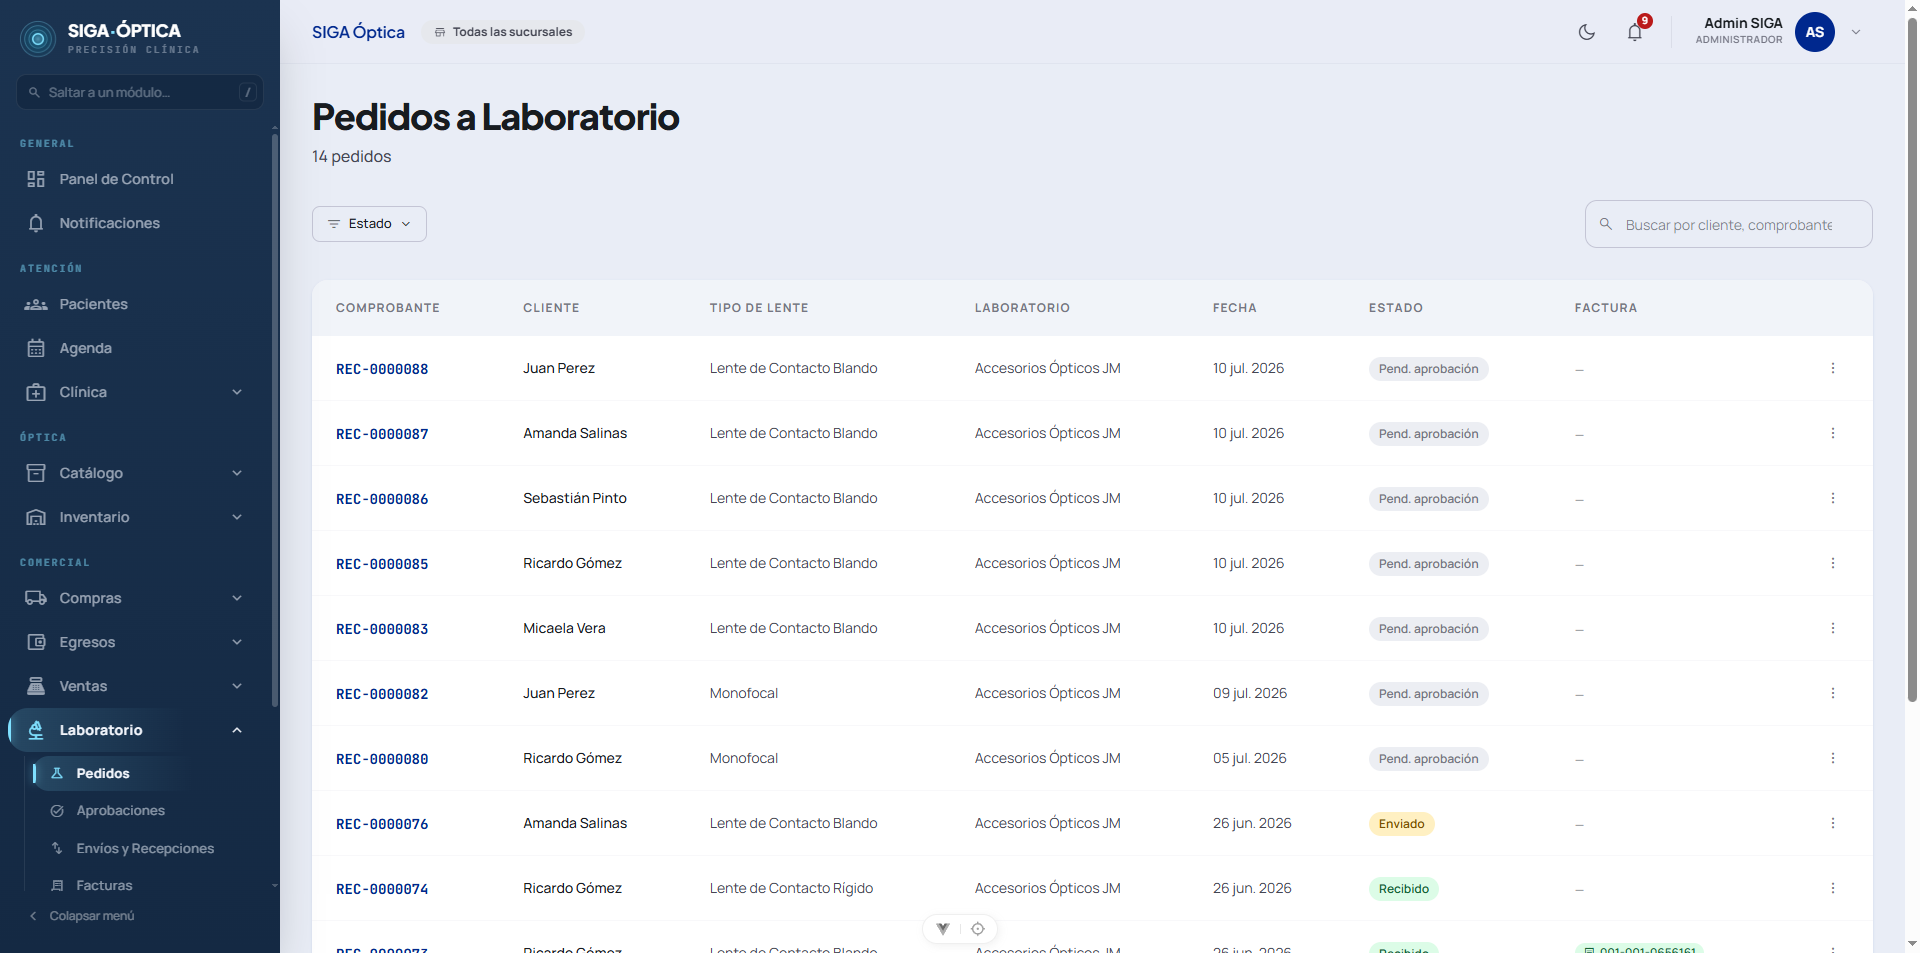
\includegraphics[width=0.95\textwidth]{imagenes/mod09-laboratorio-pedidos.png}
\caption{Cola de pedidos al laboratorio óptico externo, con el tipo de lente y su estado.}
\label{fig:mod09-laboratorio}
\end{figure}

\section{Estado}
\label{sec:lab-estado}

\Implementado\ end-to-end (backend y frontend). Sin limitaciones conocidas propias del módulo --- las limitaciones del flujo óptico en general (no poder editar receta/laboratorio de un presupuesto ya confirmado) están documentadas en el Capítulo~\ref{mod:08-ventas} (Ventas).
